\section{Vormistamine}  \label{vormistamine}
Teie lõputöö dokumendi vormistamine hõlmab väga erinevaid tööriistu, millest Te kõigest ei pruugi teadlik olla. Kuna hea vormistamine on 25\% Teie lõputöö hindest, on oluline vormistamist võtta tõsiselt ja varuda selleks aega. Eriti kui Te ei ole varem nii suuri dokumente nii põhjalikult vormistanud või vastavate tööriistade kasutamist õppinud. Käesolevas peatükis vaatame lähemalt lõputöö erinevate osade vormistamispõhimõtteid.

\subsection{Tiitel- ja infoleht}
Kõige esimese lehekülge – tiitellehe – vormistamine on siin mallis juba tehtud. Tiitellehel peab olema Teie lõpetatav õppekava (sh õppeasutus ja instituut), lõputöö pealkiri, töö liik ning maht vastavalt õppetasemele, Teie kui autori nimi, Teie töö juhendajate nimed ja teaduskraadid ning töö avaldamise asukoht ja aasta. Tiitellehele tulev info tuleb teil sisestada väljadesse failis \path{thesis.tex}. Kindlasti kontrollige kirjutatud informatsioon üle. Näiteks, kas teie juhendaja kraadi lühend on MSc (Master of Science) või MA (Master of Arts). Erinevate õppekavade lõpetajatel on kraadi nimetus erinev.

Tiitellehele järgneb infoleht (fail \path{0-info.tex}), kus on Teie töö lühikokkuvõte, võtmesõnad ning CERCS koodid. Lühikokkuvõte peaks andma ülevaate kõigist Teie töös tehtust. Näiteks kui Teie töö sisupeatükkidest kolm on sellised, mis kirjeldavad põhjalikult erinevaid töö käigus tehtud asju ning vastavaid tulemusi, siis peaks lühikokkuvõttest olema see informatsioon loetav. Keskenduge lühikokkuvõttes sellele, mida Teie tehtust saab tööst lugeda.

Võtmesõnad on teie töös olulisi komponente nimetavad mõisted, nimetused või nimed. Võtmesõnade väljamõtlemine vajab, et Te mõtleksite oma tööst ülevaatlikult. Millised olulised mõisted tulevad Teile pähe, kui Te oma tööst tervikuna mõtlete? Inspiratsiooniks on hea vaadata teisi varem sarnasel teemal tehtud lõputöid ning nende võtmesõnu. Joonis~\ref{fig:võtmesõnad} esitab varasemalt Tartu Ülikooli arvutiteaduse instituudis aastatel 2015-2021 kaitstud lõputööde populaarsemate võtmesõnade sõnapilve\footnote{\url{https://cglearn.eu/theses/top}}.

\begin{figure}[h]
    \centering
    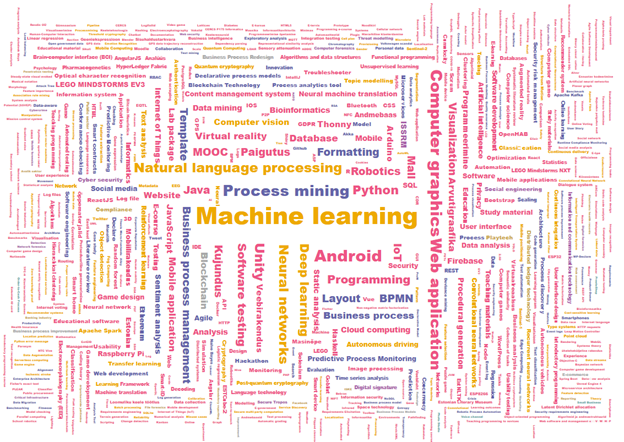
\includegraphics[width=\textwidth]{figures/Joonis1-Võtmesõnad.png}
    \caption{Aastatel 2015-2021 arvutiteaduse instituudis kaitstud lõputöödes kasutatud levinumate võtmesõnade sõnapilv.}
    \label{fig:võtmesõnad}
\end{figure}

Lisaks võtmesõnadele tuleb Teil määrata oma tööle ka Common European Research Classification Scheme (CERCS) kood. Need koodid klassifitseerivad erinevaid teadusvaldkondi. Tihti võib lõputöö puhul olla keeruline klassifitseerida seda konkreetsete CERCS klassifikaatoritega. Sellegipoolest tuleks Teil leida klassifikaator, kuhu alla Teie töö kõige rohkem läheb. Vajadusel võite kasutada töös ka mitut CERCS koodi. Klassifikaatorid leiab Eesti Teadusinfosüsteemi veebilehelt: \url{https://www.etis.ee/Portal/Classifiers/Index/26}.

Pärast infolehte on Teil võimalik lisada oma tööle ka visuaalne kokkuvõte. Selleks on üks joonis, mis kujutab asjalikult Teie töö protsessi ja tulemusi. Visuaalne kokkuvõte on väga kasulik lisa Teie tööle, sest see annab väga kiiresti edasi lugejale Teie töö olemuse. Samuti saate Te tehtud graafikat kasutada hiljem oma kaitsmisel ja töö populariseerimisel.

\subsection{Struktuur}
Teie lõputöö lugejale on oluline, et töö dokument oleks loogiliselt ja arusaadavalt ülesehitatud. Lugeja juhtimist läbi Teie lõputöö aitavad head pealkirjad, sisukord ning sisu mõistlik peatükkideks jaotamine.

\subsubsection{Pealkirjad}
Nii Teie lõputöö enda kui selle peatükkide pealkirjad on head mõelda lühikesed ja tabavad. Pikad pealkirjad võivad kanda endas liiga palju mõtteid ning võite oma lugeja kaotada juba pealkirja lugemisel. Lõputöö enda pealkiri võiks mahtuda maksimaalselt kahele reale.

Inglise keeles tuleks pealkirjad kirjutada läbiva suure algustähega. Selle osas on teatud sõnade puhul erinevaid stiile, kuid üldiselt peaksid kõik sõnad peale asesõnade algama suurtähega. Soovitame kasutada tööriista Capitalize My Title: \url{https://capitalizemytitle.com/}

Eesti keeles aga kirjutatakse ainult pealkirja kõige esimene täht suurtähena ning ülejäänud sõnad niimoodi nagu tavaliselt.

Pealkirjades tasub proovida vältida kirjavahemärkide kasutamist. Olenevalt töö olemusest võib näiteks mõttekriips olla sobilik. Näiteks, kui Te lõite tarkvaratoote, on töö pealkirjas hea mainida selle nimi ning mõttekriipsu kasutades paari sõnaga selle unikaalne väärtus. Seevastu näiteks komadega seotud lause pealkirja ei sobiks.

Need põhimõtted kehtivad ka Teie töö peatükkide pealkirjade puhul. Sisupeatükkide pealkirjad algavad numbritega. On Teie valida, kas tahate nummerdamist alustada Sissejuhatuse peatükist ja lõpetada Kokkuvõtte peatükiga, või jätate need kaks pealkirja nummerdamata. Siin mallis on Sissejuhatus ja Kokkuvõte nummerdatud. Kokkuvõtte peatükile järgnevad nummerdamata pealkirjad Viited ja Lisad. Kusjuures erinevate lisade jaoks on mõistlik jälle kasutada nummerdamist. Lisade nummerdamisel saab kasutada näiteks Rooma numbreid (Lisa I, Lisa II) või suurtähti (Lisa A, Lisa B).

Alampeatükkide nummerdus sisaldab ülempeatüki numbrit. Näiteks peatüki 2 alampeatükid on 2.1, 2.2 jne. Kusjuures punkt terve nummerduse lõpus on ainult esimese taseme pealkirjade korral. Alates kolmanda taseme alampealkirjast võib soovi korral nummerduse ära jätta. Siin mallis on pealkirjade stiilid (\verb|\section{...}|, \verb|\subsection{...}| jne) seadistatud niiviisi, et nummerdamine oleks sobilik.

\subsubsection{Sisukord}
Teie töö alguses, pärast infolehte ja visuaalset kokkuvõtet ning enne esimese peatüki algust, on sisukord. Sisukord on võikemakates tekstitöötlusprogrammides automaatselt genereeritav. Siin mallis on sisukord genereeritud käsuga \verb|\tableofcontents|. See käsk genereerib sisukorra töö sektsioonide/peatükkide (\verb|\section{...}|, \verb|\subsection{...}| jne) järgi.

\subsection{Tekst}
Lõputöö tekst peab olema rööpjoondatud (teksti äär nii vasakult kui paremalt lehe servast sirge). See võib tekitada olukorra, kus ühes reas jääb sõnade vahele visuaalselt liiga palju ruumi. Sellisel juhul tuleks kasutada poolitamist, et sõnadevahelist ruumi korrastada. Paljud tekstiredaktorid pakuvad ka automaatset poolitamiset, kuid sellega võib juhtuda, et poolitusi tuleb liiga palju. Siin mallis on LaTeX-i automaatne poolitamine minimeeritud ning kasutatud paketti \verb|microtype|, et sõnade vahele jääv ruum ei läheks liiga suureks. Sõnade poolitamine raskendab teksti lugemist ja seda võiks teha minimaalselt. Võiks vältida olukordi, kus mitu rida järjest on poolitatud.

Teksti vormistamisel on Tartu Ülikooli arvutiteaduse instituudis kaitstavate lõputööde nõuete ja hindamise dokumendis esitatud veel mitmeid teksti vormistuse reegleid. Näiteks peaks teksti reavahe olema vahemikus 1,0–1,5. Siin mallis oleme kasutanud 1,4 reavahe, mis visuaalselt vastab Microsoft Wordi 1,5 reavahele.

On võimalik kasutada kaldkirja (\verb|\emph{...}|), rasvast kirja (\verb|\textbf{...}|) jm teksti vormistamise vahendeid, et oma tekstis mõisteid ja mõtteid rõhutada. Siiski tasub näiteks rasvase kirja kasutamisega olla pigem tagasihoidlik, et Teie töö ei muutuks liiga kirjuks.

Lõike kirjutades võite jälgida, ega Teie lõigu lõppu ei jää viimasele reale ühte üksikut sõna. Sellist sõna nimetatakse orvuks sõnaks ja visuaalselt ei ole see väga kena. Orbude sõnade või ka tekstiridade (üksik tekstirida lehe üleval ääres, mille järel hakkab uus peatükk või tuleb tühi leht) kontroll on midagi, mida on mõistlik teha puhtandi vormistamisel viimasena.

\subsection{Elemendid}
Teie lõputöö väljanägemisele ja arusaamise parandamisele aitavad väga palju kaasa erinevad illustratiivsed objektid nagu joonised, tabelid ja koodinäited.

\subsubsection{Joonised}
Joonisteks nimetame kõiksuguseid lõputöösse lisatud pilte, olgu nendeks graafikud, fotod või ekraanitõmmised. Need kõik tuleb nimetada joonisteks, lisada number ja pealdis. Siin Overleaf LaTeX-i mallis käib käib see nii, et tuleb pilt laadida üles \verb|figures| kausta. Seejärel saab pilti kasutada järgneva koodiga:

\begin{minted}[escapeinside=||]{tex}
\begin{figure}[h]
    \centering
    \includegraphics[width=\textwidth]{figures/|\textbf{Joonis1-Nimi.png}|}
    \caption{|\textbf{Joonise pealdise tekst.}|}
    \label{fig:|\textbf{jooniseNimi}|}
\end{figure}
\end{minted}

Ülal koodis tuleb kirjutada \verb|figures| kaustas asuva pildifaili failinimi koos laiendiga, lühike joonise pealdise tekst ja joonisele ristviitamiseks joonise lühinimi ehk \emph{label}.

Pealdise tekstist peaks olema selge, mida on joonisel kujutatud. Pealdis tekib joonise alla ja koos elemendi sildiga „Joonis” ning automaatse joonise numbriga.

\begin{wrapfigure}{r}{0.33\textwidth}
    \centering
    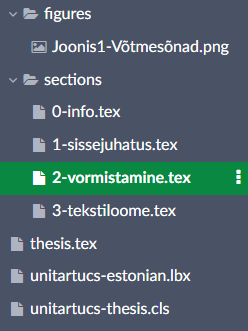
\includegraphics[width=0.33\textwidth]{figures/Joonis2-FiguresKaust.png}
    \caption{Malli kaustad.}
    \label{fig:folders}
\end{wrapfigure}

Te võite jooniseid paigutada oma töös nii lehe keskele kui ka mähkida näiteks teksti kõrvale. Tekstiga mähitud joonise loomiseks tuleb eelnenud joonise koodinäites \verb|figure| asemel kasutada \verb|wrapfigure|. Joonise laiuse võib panna näiteks \verb|width=0.33\textwidth|.

Teksti on soovitav joonise ümber mähkida olukorras, kus joonise laius on umbes 1/3 lehekülje laiusest. Muudel juhtudel näeb joonis tõenäoliselt parem välja lehekülje keskel ilma mähkimiseta.

Jooniseid paigutades tuleb olla väga ettevaatlik, et Te ei skaleeriks joonist ebaühtlaselt. Joonise suurust skaleerides muutes peab joonis nii vertikaalselt kui horisontaalselt skaleeruma samamoodi. Tüüpiliselt LaTeX-is jooniste skaleerimisel seda olukorda ei juhtu, kuid teiste programmidega joonise töötlemisel tuleb seda asjaolu silmas pidada.

Jooniseid tehes on soovitatav luua enda lõputöö jaoks ühtlane värvipalett ja stiil. See tähendab, et kui Te teete näiteks graafikuid, siis nendel oleks kasutatud läbivalt samu värve (muidugi samas tähenduses) ja stiili. Hea tööriist värvipaleti loomiseks on Coolors: \url{https://coolors.co/generate}. Vastavalt olukorrale tuleb muidugi arvestada, et Teie värvipaleti värvid toetaksid ka graafikute lugemist ning korrektset tõlgendamist. Näiteks ei tohiks valida liiga sarnaseid värve graafikul kahe sisuliselt erineva elemendi tähistamiseks. Andmete visualiseerimise põhimõtete kohta on näiteks rääkinud Tamara Munzner oma loengus Keynote on Visualization Principles~\cite{tamara_munzner_keynote_2012}. Hea ja ühtlane värvivalik ning stiil ei ole olulised mitte ainult andmete visualiseerimisel, vaid ka näiteks ekraanitõmmistele lisatud graafiliste elementide ja ka muidu jooniste puhul üldiselt.

\subsubsection{Tabelid}
Peale jooniste saab lõputöösse lisada ka andmetabeleid. Tabelite lisamisel tuleks arvestada, et väga suuri tabeleid on raske lugeda ja võib-olla peaks nendel kujutatut esitama hoopis graafikuna. Mõnikord on aga oluline andmed esitada just tabeli kujul. Väiksemad tabelid sobivad väga hästi lõputöö sisusse. Suuremad tabelid saab esitada lõputöö lisades, kas sektsioonis Lisad või isegi eraldi failina lõpuööga kaasapandud failide komplektis.

Tabeli puhul kehtivad samad soovitused nagu jooniste puhul. Ainus erinevus on, et tabeli pealdis käib tabeli kohale (jooniste puhul käib alla). Vaata näiteks tabel~\ref{tabel:elementideErinevused}.

\begin{table}[htb!]
    \centering
    \caption{Jooniste ja tabelite vormistamise erinevused lõputöö dokumendis.}
    \label{tabel:elementideErinevused}
    \begin{tabular}{|r|c|c|}
    \hline
    & \textbf{Pealdise asukoht} & \textbf{Sisu} \\
    \hline
    \textbf{Joonis} & All &   Pildid, graafikud, fotod, ekraanitõmmised \\
    \hline
    \textbf{Tabel} & \cellcolor{cellhighlight} Kohal & Andmed \\
    \hline
    \textbf{Koodinäide} & All või puudub & Programmi kood, pseudokood \\
    \hline
    \end{tabular}
\end{table}

Ülal olev tabel~\ref{tabel:elementideErinevused} on loodud järgneva koodiga:
\begin{minted}{tex}
\begin{table}[htb!]
    \centering
    \caption{Jooniste ja tabelite vormistamise erinevused lõputöö dokumendis.}
    \label{tabel:elementideErinevused}
    \begin{tabular}{|r|c|c|}
    \hline
        & \textbf{Pealdise asukoht} & \textbf{Sisu} \\
    \hline
    \textbf{Joonis} & All &   Pildid, graafikud, fotod, ekraanitõmmised \\
    \hline
    \textbf{Tabel} & \cellcolor{cellhighlight} Kohal & Andmed \\
    \hline
    \textbf{Koodinäide} & All või puudub & Programmi kood, pseudokood \\
    \hline
    \end{tabular}
\end{table}
\end{minted}

See kood on sarnane eelnelnud jooniste koodiga, kuid sisaldab kahte keskkonda. Esiteks on keskond \verb|table|, mille sees on ka tabelile eelnev pealdis. Seejärel tuleb keskkond \verb|tabular|, kus on siis juba tabel ise. Tulbad on joondatud nii, et esimene tulp on paremjoondusega \verb|r| ning teised keskjoondusega \verb|c|. Esimese tulpa ja esimese rea oleme kirjutanud rasvase kirjaga ning üks lahter on värvitud helesiniseks.

\subsubsection{Koodinäited}
Programmi kood on soovitatav kirjutada püsisammulise (\emph{monospace}) kirjastiiliga. Tuleks valida üks selline kirjastiil ja kasutada sama läbivalt lõputöö vältel. Näited sellistest püsisammulistest kirjastiilidest on Consolas ja \texttt{Courier New}. Käesolevas mallis oleme kasutanud \verb|fontspace| paketti, milles on olemas kirjastiil \texttt{Courier New}\footnote{\url{https://www.overleaf.com/learn/latex/Questions/Which_OTF_or_TTF_fonts_are_supported_via_fontspec\%3F}}.

Koodinäite vormistamine ei ole nii reguleeritud nagu piltide ja tabelite puhul. Lühikesi koodinäiteid saab kirjutada teksti sisse. Näiteks me võime kirjutada, et muutuja deklareerimine ja väärtuse omistamine käib koodiga \verb|var a = 10;|. Pikema koodinäite puhul tuleks teha eraldi plokk, näiteks nii:

\begin{minted}{javascript}
function add(a, b) {
    return a + b;
}
\end{minted}

Ülalolevas näites on kasutatud \verb|minted| keskkonda \verb|minted| paketist. See keskkond on stiliseeritud lisama koodinäitele ümber joont ja kasutama püsisammulist kirjastiili. Teatud programmeerimiskeeli oskab see pakett ka ise värvida\footnote{\url{https://www.overleaf.com/learn/latex/Code_listing\#Supported_languages}}. Koodiplokki ümbritsev tekst peab piisavalt selgelt vastavat koodi sisuliselt käsitlema.

\subsubsection{Matemaatilised valemid}
Matemaatiliste valemite vormistamine LaTeX-is on suhteliselt lihtne. Lühikese valemi kirjutamiseks teksti sisse tuleb see ümbritseda \verb|$|-märkidega. Näiteks liitmist kirjeldab valem $a+b=c$. Suurema ja viidatava valemi jaoks tuleb valem lisada \verb|equation| keskkonna sisse.
\begin{equation}
    \frac{a + b}{c} = d
    \label{eq:abcd}
\end{equation}

Ülalolev näide on tehtud koodiga:
\begin{minted}{tex}
\begin{equation}
    \frac{a + b}{c} = d
    \label{eq:abcd}
\end{equation}
\end{minted}

Nagu näha, siis valemile saab lisada ka lühinime (\emph{label}), talle tekib automaatselt number ning seda lühinime saab kasutada, et valemit numbri järgi viidata. Näiteks ülalolev näide siin mallis on numbriga~\ref{eq:abcd}.

\subsection{Viited}
Õigesti viitamine on Teie töös väga oluline. Ebaõnnestunud viitamise korral võib Teie töö sisaldada akadeemilist petturlust ning selle eest võib Teie töö saada ülevaatamisel negatiivse hinnangu. Käesolevas mallis on eelnevalt kasutatud kolme tüüpi viiteid. Nendeks on töö enda erinevate elementide ja osade vahel olevad ristviited, niinimetatud nõrkade välisviidete jaoks kasutatud joonealused viited ning kasutatud allikate põhiviited ehk tugevad viited. Ristviide muutub teksti sees ka lingiks (see link säilub ka PDF{\babelhyphen{nobreak}}faili eksportimisel). See tähendab, et kui ristviite peale vajutada, viiakse lugeja viidatud elemendi juurde.

\subsubsection{Ristviited}
Teie töös olevad joonised, tabelid ja matemaatilised valemid peavad kõik olema tekstis ristviidatud. Selle reegli eesmärk on tagada, et Teie tööd illustreerivad elemendid päriselt ka töö sisu toetaks. Lisatud element peab olema Teie tekstiga seotud ning seega õiges kohas ristviidatud. Ristviidataval elemendil peab olema lühinimi (\emph{label}) ja selle nimega saab luua ristviite käsuga \verb|\ref{lühinimi}|. Viiteks tuleb elemendi järjekorranumber, mis muutub teksti sees lingiks (see link säilub ka PDF-faili eksportimisel). See tähendab, et kui ristviite peale vajutada, viiakse lugeja viidatud elemendi juurde.

\subsubsection{Joonealused viited}
Väliseid viiteid saab nimetada nõrkadeks ja tugevateks. See kirjeldus ei ütle midagi välise viite mõju või kasulikkuse kohta Teie tööle. Tihtipeale on teatud väliste viidete puhul ka vaja teha Teil subjektiivne otsus, kas see on pigem nn nõrk või tugev viide. Nõrgad viited on näiteks viited Wikipedia artiklitele, Stack Overflow postitustele, toodete kodulehtedele, sõnastikele ja privaatsele suhtlusele, kus viidatud allikas ei ole väga selgelt konkreetse autori poolt mõnes väljaandes publitseeritud. Üldiselt võib mõelda, et kõiksugused veebiviited on just pigem nõrgad viited. Samas veebiviide võib olla ka näiteks tunnustatud autori poolt kirjutatud blogipostitus, mis juhul võib tegu olla pigem tugeva viitega.

Nõrgad viited tuleks vormistada joonealuste viidetena. Selleks tuleb kasutada käsku \verb|\footnote{...}| ja selle sisse kopeerida veebiviite link. Selleks, et link muutuks ka päriselt õigesti vormistatud lingiks, oleme teinud siia malli käsu \verb|\url{...}|. Ehk siis lingi lisamine joonealuseks viiteks oleks \verb|\footnote{\url{...}}|. Sellise viite puhul ei ole väga oluline hakata viitesse otsima autorit (nt mõne toote veebilehe, tarkvara dokumentatsiooni või Wikipedia artikli puhul ei pruugigi olla lihtsasti tuvastatavat autorit). Tüüpiliselt piisab lisada joone alla lihtsalt link vastavale veebilehele, kust Te viidatud info saite.

Sellised joonealused viited on väga head, kuid Teie töö peaks põhinema lisaks nendele ka mõistlikul hulgas tugevatel viidetel ehk põhiviidetel.

\subsubsection{Põhiviited}
Siin mallis nimetame põhiviideteks neid viiteid, mis lähevad Teie töö lõpus olevasse Viidete sektsiooni. Seda sektsiooni nimetatakse vahel ka „Viidatud kirjandus“ või „Kasutatud allikad“. Sinna lähevad tugevad viited, mis on tüüpiliselt konkreetse autori poolt tunnustatud väljaandena avaldatud. Näiteks teadusartiklid, raamatud, konverentsiettekanded, lõputööd, aga ka võivad olla blogipostitused või uudisartiklid. Vastavalt Teie õppeastmele, millel lõputööd esitate, võiks Teil põhiviiteid olla piisavalt. Täpset arvu on keeruline öelda, sest see sõltub palju Teie töö olemusest, viidatud allikate tugevusest ning kui põhjalikult olete viiteid kasutanud. Samas võib öelda, et näiteks ainult kaks põhiviidet on iga kõrghariduse õppeastme puhul kindlasti liiga vähe.

Põhiviidete vormistamisel on levinud erinevates valdkondades levinud erinevad stiilid. Oma lõputöös on Teil võimalik valida omale meeldiv viitamisstiil. Arvutiteaduses on väga levinud ACM ja IEEE numbrilise viitamise stiilid. Need on sellised, kus allikad nummerdatakse nurksulgudes olevate numbritega (nt „[1]“, „[2]“ jne) ja nendega ka teksti sees viidatakse. Matemaatikas on levinud ka trigraafiline AMS viitamisstiil, kus nurksulgude sees on autorite esitähed või initsiaalid ning osa aastanumbrist (nt „[Mun12]“). Sotisaalteadustes on pigem levinud näiteks APA stiil, kus viidatakse autori nime ja aastaarvuga (nt „(Munzner, 2012)“).

Viidete vormistamiseks on siin mallis kasutatud \verb|biblatex| paketti. See pakett võimaldab Teil lihtsasti lisada oma viited, neile viidata ja muuta viitamisstiili. Käesoleva malli põhifailis \verb|thesis.tex| on \verb|biblatex| sisselaadimise käsk. Seal sees on vaikimisi seadistatud IEEE numbriline viitamisstiil. Võite vaadata, mis stiile \verb|biblatex| pakett veel toetab ja valida omale meelepärase: \url{https://www.overleaf.com/learn/latex/Biblatex_citation_styles\#Citation_styles}.

Lisaks viitamisele on Teil vajalik saada ka viidatavate allikate bibliograafia kirjed LaTeX-i. Selleks soovitame kasutada viidete haldamise tööriista Zotero\footnote{\url{https://www.zotero.org/}}. Zotero võimaldab Teil koguda viited ja nendega seotud andmed (sh failid ja Teie märkmed) väga lihtsasti Teie isiklikku andmebaasi Zotero töölauarakenduses. Juba näiteks mustandi kirjutamisel Google Docsis on Teil võimalik Zoterot kasutada, et viited õigetesse kohtadesse lisada ja vormistada.

Overleaf LaTaX-i vormistama tulles saate Zoterost eksportida vajalikud bibliograafiakirjed. Selleks selekteerige Zoteros oma lõputööga seotud viited ning valige kontekstimenüüst \emph{Export Items...} (vt joonis~\ref{fig:zoteroKontekst}). Avanevast menüüst valige ekspordi formaadiks \verb|BibLaTeX|.

\begin{figure}[htb!]
    \centering
    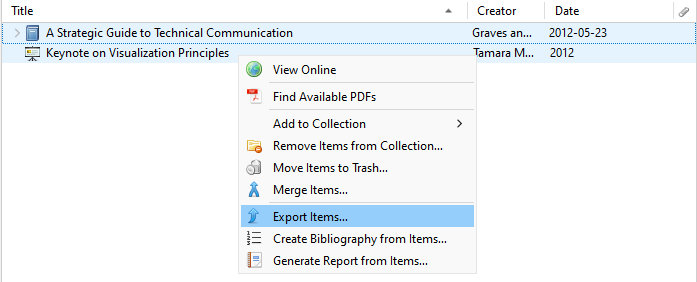
\includegraphics[width=\textwidth]{figures/Joonis3-ZoteroBibliograafiaEksport.png}
    \caption{Valitud allikate kontekstimenüü Zotero programmis.}
    \label{fig:zoteroKontekst}
\end{figure}

Seejärel Zotero ekspordib teie valitud allikate kirjed \verb|.bib| faili, mille sisu saate tõsta Overleaf keskkonda faili \verb|viited.bib| ning seejärel nende allikate viitamine juba töötabki. Igale allikale loob Zotero lühinime, millega saate viidata. Näiteks siin mallis Tamara Munzneri loengule viitamiseks on kasutatud käsku \verb|\cite{tamara_munzner_keynote_2012}|.

Viidatud teadusartiklitel on tüüpiliselt Document Object Identifier (DOI) numbrid. Nende põhjal tekivad DOI lingid  (kujul doi.org/[number]). Teadusartiklitele viidates on soovitatav lisada viitesse ka vastavad DOI lingid ilma vaatamise kuupäevata. Allikate linkide lisamisel tuleb kindlasti tähele panna, et on õiged ja töötavad lingid. Võib juhtuda olukord, kus kasutate teadusartiklitele ligipääsuks ülikooli vaheserverit (\emph{proxy}) ja sellisel juhul võivad Teie lingid veebilehitseja aadressiribal olla selle vaheserveri lingid. Kontrollige kindlasti, et allikate lingid oleksid puhtad, töötavad ning võimalusel eelistage DOI linke.

\subsection{Lisad}
Pärast viidete sektsiooni tuleb Teie lõputöös sektsioon “Lisad”. Selles sektsioonis saab esitada näiteks suuremad tabelid või ekraanitõmmised, mis töö sisu osasse ei mahu. Tihtipeale on seal mõistlik ka esitada Teie tööga seotud sõnastik, kus olete defineerinud oma töös kasutatud spetsiifilised erialaterminid. Olukorras, kus olete lõputöö käigus loonud tarkvara, saab sektsiooni “Lisad” lisada ka tarkvara käivitus- ja kasutusjuhendi. Iga nimetatud lisa kohta saab sektsiooni “Lisad” teha eraldi alajaotuse ja omale meeldival viisil need nummerdada. Näiteks: „Lisa I: Sõnastik“, „Lisa B – Programmi kasutusjuhend“ vms. Juhiseid hea kasutusjuhendi kirjutamiseks on mitmeid, kuid üks soovitus on näiteks Graves ja Gravesi õpik „A Strategic Guide to Technical Communication“ tehnilist laadi teksti kirjutamiseks~\cite{graves_strategic_2012}.

Väga oluline lisa on kaasapandud failide kirjeldus. Lõputöö enda dokumendiga koos on Teil võimalik esitada arhiivifail. Seal arhiivifailis on tüüpiliselt pikemad tekstid (nt kui programmi kasutusjuhend on pikk, on vaja olnud lisada pikemad kasutatud varade litsentsid, uuringus kasutatud küsimustik vms), suuremad andmefailid (nt uuringu käigus mõõdetud analüüsimata tulemused, nende tulemuste analüüsifailid, heli- ja videosalvestised tarkvarast või selle testimisest vms), loodud tarkvara, selle lähtekood, disaini kontseptsioonid ja muud Teie lõputöö käigus tekkinud failid. Lisade sektsioonis kasutage ühte lisadest, et kirjeldada kaasapandud arhiivi sisu.

\subsection{Litsents} \label{subchapter:litsents}
Pärast sektsiooni “Lisad” tuleb Teie lõputöö dokumendi kõige lõppu lisada litsents, mis lubab Tartu Ülikoolil säilitada ja avaldada Teie lõputööd. Selle teksti uuendatakse tihti ja võib sõltuda sellest, kas Teie lõputöö tekst on salastatud või mitte. Uusimad litsentsi tekstid leiate: \url{https://adr.ut.ee/?page=pub_list_dynobj&desktop=57835&tid=70993&data_only=true&search=Otsi&field_100193_search_type=ANY&field_100193_text_search_value=ppimine}

Ülaoleval lingil on lihtlitsents dokumendis numbriga 30. Enamikel juhtudest peaks see litsents Teile sobima. Olukorras, kus Teie töö sisaldab informatsiooni, mida ei tohi mingi ajaperioodi jooksul või isegi tähtajatult avaldada, peate esitama vastava litsentsi kasutamiseks avalduse õppeprodekaanile. Avaldus on dokumendis number 32 ja kui õppeprodekaan on Teie avalduse rahuldanud, saate kasutada vastavate piirangutega litsentsi dokumendist numbriga 31.

\subsection{Meta-andmed}
Teie lõputöö faili küljes on ka meta-andmed ehk andmed lõputöö faili kohta. Käesolev mall lisab need Teie tööle automaatselt \verb|thesis.tex| failis täidetud andmeväljade pealt. PDF faili meta-andmeid saate näha näiteks tarkvaraga Acrobat Reader, kui valite avatud dokuemndi kontekstimenüüst \emph{Document Properties} (vt joonis~\ref{fig:metaAndmed}). On oluline, et Teie töö meta-andmed vastaksid tegelikkusele.

\begin{figure}[htb!]
    \centering
    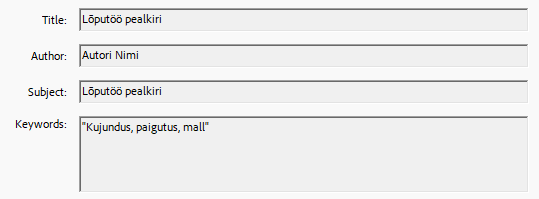
\includegraphics[width=0.8\textwidth]{figures/Joonis4-MetaAndmed.png}
    \caption{Malli meta-andmed Acrobat Reader programmis.}
    \label{fig:metaAndmed}
\end{figure}

Soovitame üle vaadata üle kõiksugused failiga seotud meta-andmed, et nendes ei oleks midagi ebakorrapäratut. Varasemalt on juhtunud, et meta-andmetes olev faili autor ei ole olnud lõputöö tegelik autor. Selline vastuolu tekitab kahtlust, kes on lõputöö dokumendi tegelikult kirjutanud.
